%%%%%%%%%%%%%%%%%%%%%%%%%%%%%%%%%%%%%
% Preamble for defining document properties
%%%%%%%%%%%%%%%%%%%%%%%%%%%%%%%%%%%%%
%%%%%%%%%%%%%%%%%%%%%%%%%%%%%%%%%%%%%
% Template for LCA-EPFL Students Report
%%%%%%%%%%%%%%%%%%%%%%%%%%%%%%%%%%%%%

\documentclass[11pt, a4paper, twoside]{report}

%%%%%%%%%%%%%%%%%%%%%%%%%%%%%%%%%%%%%
% Packages
%%%%%%%%%%%%%%%%%%%%%%%%%%%%%%%%%%%%%
\usepackage[applemac]{inputenc}
\usepackage{graphicx}
\usepackage{fullpage}
\usepackage{epsfig}
\usepackage{listings}
\usepackage{amsmath}
\usepackage{subfigure}
\usepackage{nomencl}
% For customizing header and footers
\usepackage{fancyhdr}
\usepackage{lscape}
\usepackage{algorithm}
\usepackage{algorithmic}
\usepackage{color}
\usepackage{dirtree}
\usepackage{hyperref}

%%%%%%%%%%%%%%%%%%%%%%%%%%%%%%%%%%%%%
% Customizing headers and footers
%%%%%%%%%%%%%%%%%%%%%%%%%%%%%%%%%%%%%
\pagestyle{fancyplain}

%\fancypagestyle{plain}{  }

\renewcommand{\headrulewidth}{0pt}
\newcommand{\tit}{}
\newcommand{\aut}{FirstName LastNAme}
\renewcommand{\sectionmark}[1]{ \markright{\thesection.\ #1}}

% Header
\rhead[\fancyplain{}{} ] {\textbf{\fancyplain{ \nouppercase{\rightmark} \hspace{1cm} \thepage } { \nouppercase{\rightmark}\hspace{1cm} \thepage } }}
\chead[\fancyplain{}{} ] {\fancyplain{}{} }
\lhead[\textbf{\fancyplain{\thepage \hspace{1cm} \nouppercase{\leftmark} }{\thepage \hspace{1cm} \nouppercase{\leftmark}} }]{\fancyplain{}{} }
%Footer
\lfoot[\fancyplain{\tit}{\tit}] {\fancyplain{}{}}
\cfoot[\fancyplain{}{}] {\fancyplain{}{}}
\rfoot[\fancyplain{}{}] {\fancyplain{\tit}{\tit}}

\setlength{\headsep}{0.6cm}

%%%%%%%%%%%%%%%%%%%%%%%%%%%%%%%%%%%%%
% For code insertion
%%%%%%%%%%%%%%%%%%%%%%%%%%%%%%%%%%%%%
% "define" Scala
\lstdefinelanguage{scala}{
  morekeywords={abstract,case,catch,class,def,%
    do,else,extends,false,final,finally,%
    for,if,implicit,import,match,mixin,%
    new,null,object,override,package,%
    private,protected,requires,return,sealed,%
    super,this,throw,trait,true,try,%
    type,val,var,while,with,yield},
  otherkeywords={=>,<-,<\%,<:,>:,\#,@},
  sensitive=true,
  morecomment=[l]{//},
  morecomment=[n]{/*}{*/},
  morestring=[b]",
  morestring=[b]',
  morestring=[b]"""
}


\definecolor{dkgreen}{rgb}{0,0.6,0}
\definecolor{gray}{rgb}{0.5,0.5,0.5}
\definecolor{mauve}{rgb}{0.58,0,0.82}
 
% Default settings for code listings
\lstset{frame=tb,
  language=scala,
  aboveskip=3mm,
  belowskip=3mm,
  showstringspaces=false,
  columns=flexible,
  basicstyle={\small\ttfamily},
  numbers=none,
  numberstyle=\tiny\color{gray},
  keywordstyle=\color{blue},
  commentstyle=\color{dkgreen},
  stringstyle=\color{mauve},
  frame=single,
  breaklines=true,
  breakatwhitespace=true
  tabsize=3
}

\makeglossary
\renewcommand{\nomname}{List of Acronyms}

%makeindex PDMReport.glo -s nomencl.ist -o PDMReport.gls

\usepackage{multirow}

\graphicspath{{images/}}

% begin latex document
\begin{document}

%%%%%%%%%%%%%%%%%%%%%%%%%%%%%%%%%%%%%
% Title page
%%%%%%%%%%%%%%%%%%%%%%%%%%%%%%%%%%%%%
\newcommand{\logoepfl}[0]{\vspace*{1.5cm}\begin{center}
\includegraphics[scale=0.4,keepaspectratio=true]{images/EPFL.pdf}\end{center}\hrule\vspace{1cm}}

\newcommand{\project}[1]{\begin{center}\large{#1}\end{center}}
\renewcommand{\title}[1]{\vspace{0.01cm}\begin{center}\LARGE{#1}\end{center}\vspace{0.2cm}}
\renewcommand{\author}[1]{\begin{center}\Large{#1}\end{center}}
\newcommand{\department}[1]{\begin{center}\large{#1}\end{center}}
\renewcommand{\date}[2]{\begin{center}\normalsize{#1 #2}\end{center}}

\newcommand{\supervisor}[4]{\begin{center}\begin{normalsize}{\bf #1}\\#2\\#3\\#4\end{normalsize}\end{center}}


\thispagestyle{empty}

\logoepfl

\project{Studyplan Visualisation}
\title{Project Documentation}
\author{Christopher Chiche \\ Julien Perrochet}
\department{CRAFT \\ EPFL}
\date{\today}

\begin{center}
\begin{tabular}{cc}
\begin{tabular}{p{6cm}}
\supervisor{Supervisor}{Pierre Dillenbourg}{EPFL}{CH-1015, Lausanne}
\end{tabular}
\end{tabular}
\end{center}

\clearpage \thispagestyle{empty} \cleardoublepage


%%%%%%%%%%%%%%%%%%%%%%%%%%%%%%%%%%%%%
% Dedication page
%%%%%%%%%%%%%%%%%%%%%%%%%%%%%%%%%%%%%
%\include{dedication}

% Start roman numbering
\pagenumbering{roman} \setcounter{page}{1}

%%%%%%%%%%%%%%%%%%%%%%%%%%%%%%%%
% SECTION : TABLE OF CONTENT
%%%%%%%%%%%%%%%%%%%%%%%%%%%%%%%%
\renewcommand{\contentsname}{Table of Contents}
\tableofcontents
\clearpage
\thispagestyle{empty}
\cleardoublepage

% Set to arabic numbering after this
\pagenumbering{arabic} \setcounter{page}{1}

%%%%%%%%%%%%%%%%%%%%%%%%%%%%%%%%
% SECTION : INTRODUCTION
%%%%%%%%%%%%%%%%%%%%%%%%%%%%%%%%
\chapter{Introduction}
\section{About}
This project's original motivation was to explore the study plans proposed by each section based on actual student choices -- analysing what course students took -- instead of the standard course prerequisites and descriptions that are generally available, and to offer a tool to allow anybody to take a look at the data for himself.

To do so required two important steps:
\begin{itemize}
\item Represent the students study history with a useful model;
\item Find good visual representations for the available data.
\end{itemize}

Both steps were achieved and solid foundations were lain to enable the implementation of new visualisations.

\newpage
\section{Project Directory Structure}
We use sbt to build the code, and hence stick to its structure. Furthermore, the \verb|view|, \verb|core| and \verb|import| segments of the application each live in their own sbt sub-project.

The relevant directories are listed hereafter:

\dirtree{%
.0 .
.1 core/.
.2 src/main/.
.3 scala/.
.4 ch/epfl/recom.
.5 graph/.
.5 model/.
.6 administration/.
.5 processing/.
.6 maps/.
.7 assist/.
.5 storage/.
.6 db/.
.6 maps/.
.5 util/.
.3 plpgsql/.
.3 sqlview/.
.1 import/.
.2 src/main/scala/.
.3 ch/epfl/craft/recom/dimport/isa/.
.1 view/.
.2 src/main/scala/.
.3 ch/epfl/craft/recom/.
.4 view/.
.5 model/.
.5 snippet/.
.6 draw/.
.5 util/.
.5 view/.
}

\chapter{Model}
The model is built around the students and their course history, and this is reflected at the database level. Whenever going through the model is useless (most of the cases that were implemented), the data is accessed and processed directly through stored procedures.

For further in-depth data-mining where individual course histories must be analyzed, we believe the model will prove useful.

\section{Classes}
A few of the main classes are mentioned hereafter. They are meant to give you a glimpse of the model: for any of the classes referenced within, please refer to the project's Scaladoc\footnote{\url{http://shastick.github.com/orgarec/doc/core/\#package}}.
and to the source code\footnote{\url{https://github.com/Shastick/orgarec}}.
\begin{multicols}{2}
\begin{lstlisting}[language=Scala]
class Topic(
    val id: String,
    val name: String,
    val section: Section,
    val prerequisites_id: Set[Topic.TopicID],
    val description: 
    	Option[String],
    val credits: Option[Int]
)
\end{lstlisting}

\begin{lstlisting}[language=Scala]
class Student(
    val id: Student.StudentID,
    val arrival: AcademicSemester,
    val section: Option[Section],
    val currentSemester: Option[AcademicSemester],
    val semesterHistory: Set[AcademicSemester],
    val courses: Set[TakenCourse]   
)
\end{lstlisting}

\columnbreak
\begin{lstlisting}[language=Scala]
class Course(
    id: String,
    name: String,
    section: Section,
    prerequisites_id: Set[Topic.TopicID],
    description: Option[String],
    credits: Option[Int],
    val semester: Semester,
    val head: Head
) extends Topic
\end{lstlisting}
\begin{lstlisting}[language=Scala]
case class TakenCourse(course: Course,
    count: Int,
    grade: Option[Int],
    evaluation: Option[Int],
    semester: AcademicSemester
)
\end{lstlisting}

\end{multicols}

\section{Database Structure}
The storage layer and structure are mainly defined through Lift's Mapper. Only for the processing and data extraction have stored procedures been written, and tables added manually. Figure~\ref{fig:db_schema} shows the database schema.

To avoid confusion with class names, the database entities representing objects are suffixed with \verb|map|: a \verb|Student| object is stored in the \verb|studentmap| table.

\begin{figure}
\center
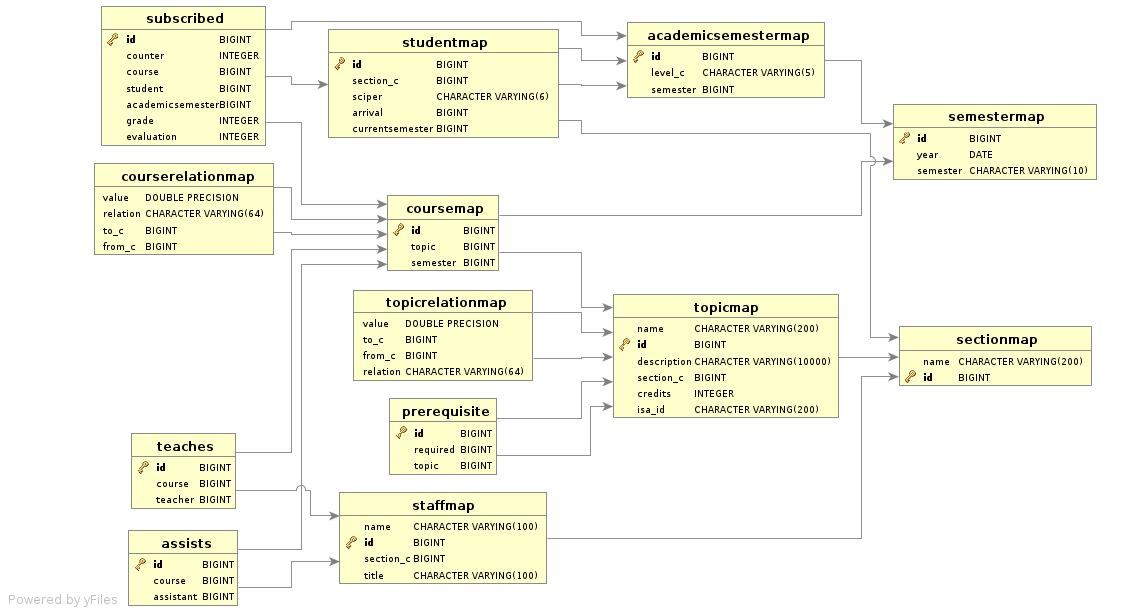
\includegraphics[angle=-90, width=.85\columnwidth]{schema_extended.png}
\caption{database schema}
\label{fig:db_schema}
\end{figure}

\subsection{Stored Procedures}
The following stored procedures are already available:
\paragraph{computeCostudents}
Populates the \verb|courserelationmap| table with the co-students count between any two courses.

\paragraph{sectionPerTopicDetail} Gets details about section participation in each topic given by a section and during which academic level.

Example: \verb|SELECT sectionPerTopicDetail| ('{SHS}'::varchar[],'{MA1,MA3}'::varchar[],\\'2012-07-01','2012-07-01')

Returns: the topic isa\_id and name, the section participating in this topic (NOT the one teaching it),
the average participating students from the section and the total number of students in this topic.
these two last numbers are averaged over the number of courses that were considered in the query
(if a span greater that 1 semester is provided, several occurences of the same topic will be counted.) 
students not in the specified academic leves (here: MA1, MA3) are not counted.

\paragraph{sectionTopics} Returns the topics teached by the specified sections

usage: \verb|sectionTopics('{IN,SC}'::varchar[])|

\paragraph{sectionTopicsWStudentCount} Return the topics teached by the specified sections, and the quantity of students that attended during the specified period.

usage: \verb|sectionTopics('{IN,SC}'::varchar[],'2011-07-01','2012-07-01')|

\paragraph{topicCostudentsSemFilter} get the costudents quantity between any two topics taught by the specified sections during the specified time interval and at the specified academic level.

usage : select \verb|topicCostudents|('{SC,IN}'::varchar[],'{BA1}'::varchar[],
'2011-07-01','2012-07-01)

\paragraph{topicCostudents} Get the costudents quantity between two topics taught by the specified section during the specified time interval

usage : select topicCostudents('{SC,IN}'::varchar[],'2011-07-01','2012-07-01)

\paragraph{topicSectionRatio} Returns the sections present in this course and the corresponding ratio. The ratio is averaged over the number of courses that occurred in the given time interval.

usage: select \verb|topicsectionratio(<isa_id>,'2011-07-01','2012-07-01)|

\chapter{Visualisation}

\section{Technology}
The web application and data serving use Lift, which is also Scala based, enabling an easy integration with the core.

JavaScript is extensively used for the actual browser-side visualization. The D3.js\footnote{www.d3js.org} library provides advanced and complete visualization tools. 

\section{Implemented visualisations}
The final version of our project includes two different visualization types. The first one, which was the primary objective of the project, represents a force directed graph\footnote{https://github.com/mbostock/d3/wiki/Force-Layout} of topics which are linked by their relations. The second type of representation, which was thought to be useful to explore SHS courses, helps representing the repartition of students in courses given their section using a Sankey diagram\footnote{https://github.com/d3/d3-plugins/tree/master/sankey}. 

\subsection{Organic graph of courses}
This visualization is meant to easily visualize the relationship between various courses and the study plan. In this project we use only the percentage of students taking two courses to evaluate their distance, the more co-students they have, the closer they will be.  

\paragraph{Key principles}
In this visualization, courses are represented as nodes in a graph, while their relations are represented as links between the nodes. 

Here are the parameters we represent and how we represent them: 
\begin{description}
\item[Credits:] size of the node ;
\item[Costudents] (The percentage of students following two classes): length and width of the link.
\end{description}

The settings tab enables to choose easily which study plans we want to represent using the following parameters: 
\begin{description}
\item[Sections:] the sections from which we want to show the courses;
\item[Semesters:] the time range we want to consider;
\item[Acedemic Semester:] the academic level (BA1, MA3,...) of the students taking the courses.
\end{description}

It is also possible to modify the minimum number of co-students required to show an edge between two classes in order to generate a lighter or more complete graph. 

\paragraph{Displaying more information on courses}
When a course is selected (either by putting the mouse on the node or by using the search tool), some additional information (if available) is displayed on the lower left corner of the screen. For now, in this additional information field, there is a graph showing the most related classes (by number of co-students) and the sections of students following this class. Course links' are also highlighted in red and the size of the course node is doubled to improve its visibility.

These bar plots give a more precise information on a specific class than the original graph but would be less useful if we used only them. 

\paragraph{Search tool}
On the upper right corner of the page, there is a search tool allowing for quick class lookups using auto-complete. This feature was implemented after the user study, conducted in the end of the semester, showed that it was the most requested feature. 

\paragraph{Overview}
\begin{figure}[H]
\centering
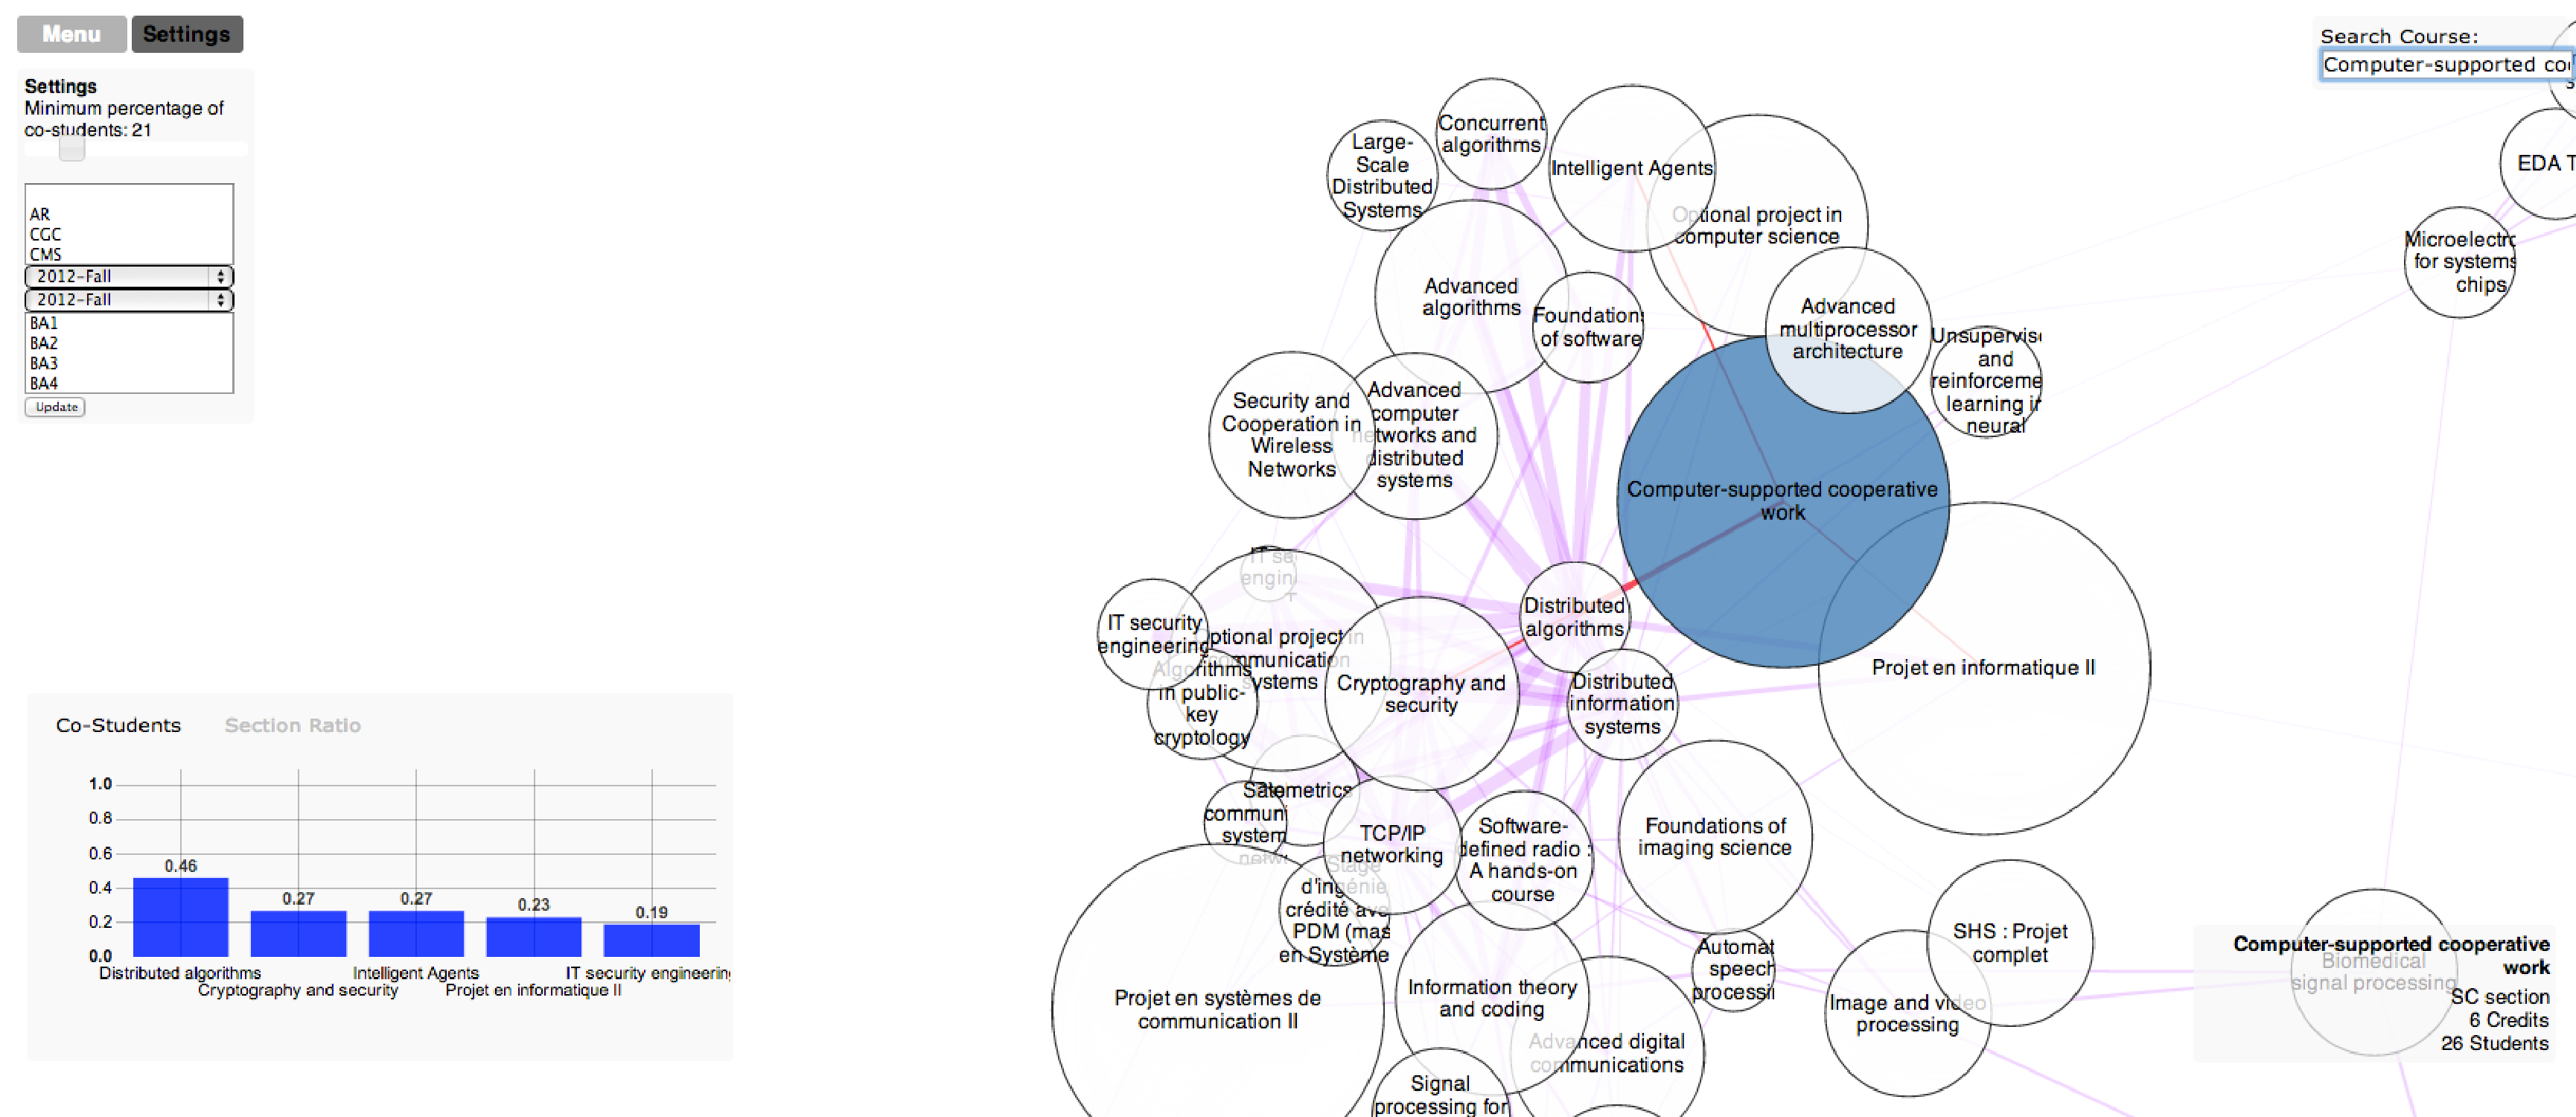
\includegraphics[width=\textwidth]{images/view_orga_global}
\label{fig:global}
\caption{Graph explorer page}
\end{figure}


\begin{figure}[H]
\centering
\subfigure[Settings]{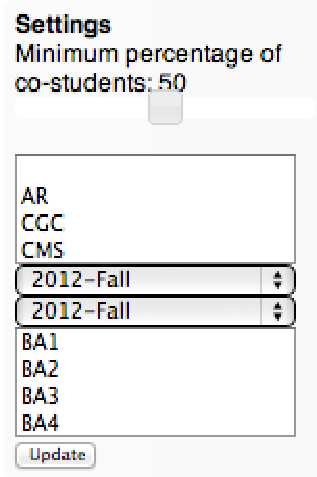
\includegraphics[height=5cm]{images/view_orga_settings}}
\subfigure[Search]{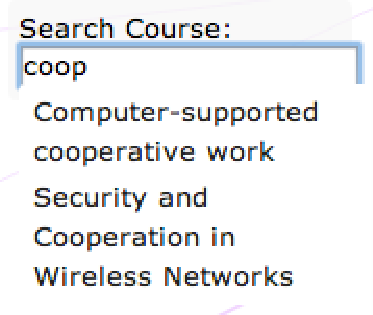
\includegraphics[height=4cm]{images/view_orga_search2}}
\subfigure[Details]{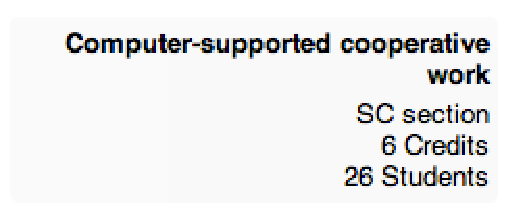
\includegraphics[height=3cm]{images/view_orga_details}}
\label{fig:orga_panels}
\caption{Panels in Graph explorer}
\end{figure}

\begin{figure}[H]
\centering
\subfigure[Co-students]{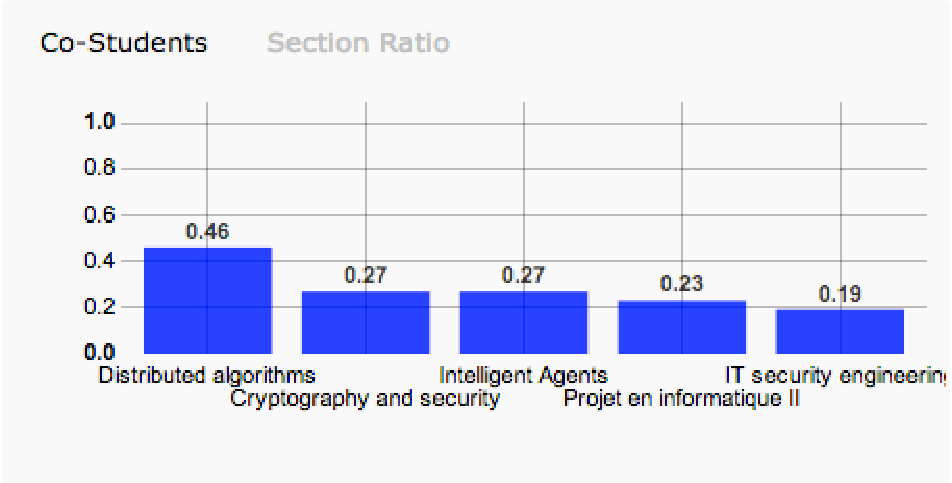
\includegraphics[height=5cm]{images/view_orga_sub_costud}}
\subfigure[Section of origin]{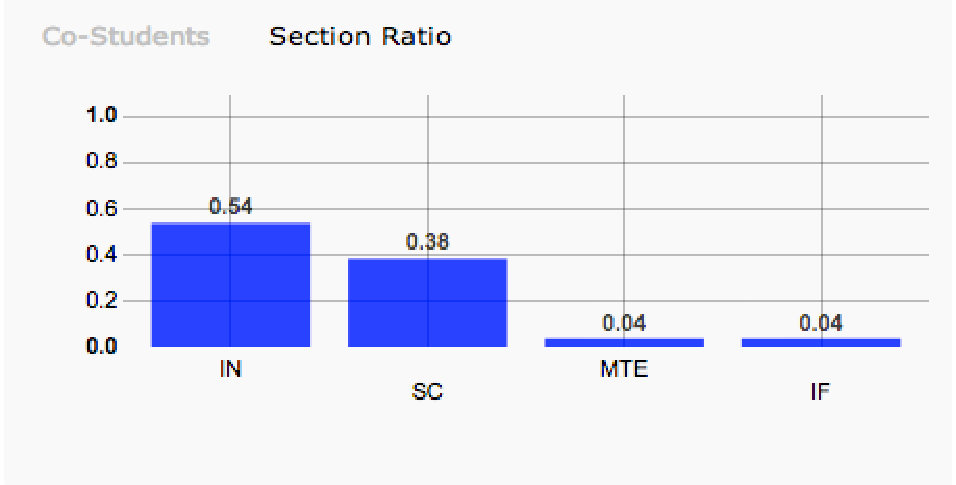
\includegraphics[height=5cm]{images/view_orga_sub_section}}
\label{fig:orga_subgraphs}
\caption{Subgraphs in Graph explorer}
\end{figure}



\paragraph{What can be added}
In the main graph it is possible to represent data using many parameters. 

For nodes we have (if we consider that nodes are circles, but we can also change the shape):
\begin{itemize}
\item Radius/Stroke width
\item Color/Stroke color
\item Opacity
\end{itemize}

For edges we have: 
\begin{itemize}
\item Length/Stroke width
\item Color/Stroke color
\item Opacity
\end{itemize}

The length of an edge is an approximation, as it is often impossible to generate a graph with arbitrary lengths for all relations. The force directed layout, however, provides a great replacement. 

\subsection{SHS explorer/Section explorer}
The section explorer considers the repartition of students from different sections in courses as a flow. The goal of this graph is to easily visualize which  courses are the most popular,  in terms of which sections the students following them are in.

\begin{figure}[H]
\centering
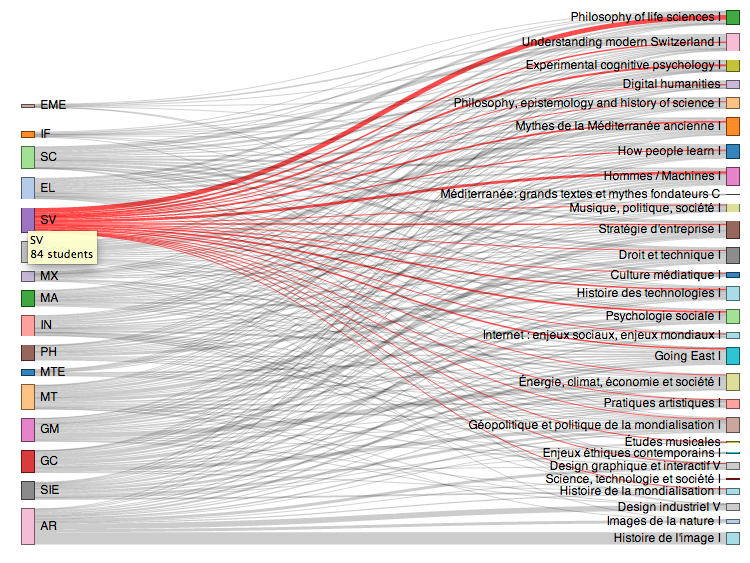
\includegraphics[width=\textwidth]{images/view_shs_SV}
\label{fig:global}
\caption{Section explorer for SHS}
\end{figure}

\section{User study}
A user study was conducted among 16 students of the IC faculty and particularly of the Computer Supported Cooperative Work course.  

The most recurrent remark was that it was really hard to find a particular course on the graph, that is why we implemented the autocomplete search tool.

\subsection{Quantitative analysis}
Table \ref{tab:userstudy} shows the results for quantitative questions. The first remark that we can make out of these results is that users did not see how this application could help them make decisions about their study plan and this even if they found the information displayed relevant and easy to access. We can also see that users did not find any use in the section/shs explorer. 
\begin{table}[H]
\center
\begin{tabular}{|c|l|c|}
\hline 
Category & \multicolumn{1}{|c|}{Question} & Mean (1-5)\\
\hline
\multirow{2}{*}{General} 
	& Does the presented information seem relevant to you? & 3.54 \\
	& Did you find it easy to browse and use the app' & 3.54 \\
\hline
\multirow{4}{*}{Course explorer}
	& Did you identify clusters representing your study experience? & 3.46 \\
	& Was it easy to find a class? & 3.30 \\
	& Would it help you choose a speciality/optional class & 2.77 \\
	& Are the additional graphs related to specific classes useful? & 2.69\\
\hline
\multirow{4}{*}{Section explorer}
	& Does the representation hold relevant information? & 3.62 \\
	& Would it help you find an interesting SHS/optional class & 2.69 \\
	& Would you choose your SHS based on this kind of graphs& 2.84 \\
\hline
\end{tabular}
\label{tab:userstudy}
\caption{Grades given by testers, from 1 (not a all) to 5 (strongly)}
\end{table}

\subsection{Qualitative analysis}

\begin{description}
\item[Course Explorer] \quad 
	\begin{itemize}
	\item \emph{Some data is wrong concerning the years where classes are given}
	\item \emph{Nodes displayed as circles should be thought again: not enough space for text}
	\item \emph{I don't understand how it works. There is not enough information.}
	\end{itemize}
\item[Section Explorer] \quad 
	\begin{itemize}
	\item \emph{I don't really understand what it represents, some information would be great}
	\item \emph{I can see where my colleagues from my section go}
	\item \emph{I think that representing section versus courses is good, but I choose my courses given my interests, not given other peoples choices}
	\item \emph{You should add the description of the class and the grading policy}
	\item \emph{It would be interesting to have previously chosen SHS, bra size + Relationship status.}
	\item \emph{Relation with hobbies and what people want to do after EPFL}
	\end{itemize}
\item[General remarks] \quad
	\begin{itemize}
	\item \emph{The visualizations are great but I am not sure that it is necessary}
	\item \emph{This application would be more suited for the board and commissions than for students}
	\end{itemize}
\end{description}

\subsection{Conclusion of the user study}

The comments show that the testers had difficulties to understand how the visualizations worked and what they represented. It is thus necessary to implement a \emph{help} button. 

The course explorer is appreciated and representative of students experience but students don't see how it can help them in their exploration of the study plan. It would be interesting to get the feedback of board members to know if it can help them better understand the study plan structure in practice.

The section explorer is less appreciated than the course explorer. When creating it we thought that it would be the most helpful representation: the study however showed us that we were wrong and that people, aside from the fact that it represents some interesting relations, don't find it useful. 

\chapter{Import}
The \verb|import| project is quite small, but holds a few key urls where data can be obtained from is-academia. As the interface to access the data is currently evolving, a straightforward importation method has not been implemented.

Scala allows easy basic XML manipulation, and examples can be found in the \verb|ISAxmlImporter| object.

\section{ISA interfaces}
The current interface IS-Academia is actually working on can be found here: \url{https://isanwww1.epfl.ch:8443/site-1.0/}. This is currently a Beta and might hence change quite rapidly.

\subsection{Legacy URLs}
These URLs were used at the beginning of the semester to build the first database draft. It is unclear if they will still be available in the future, and they are available even from the outside of EPFL's network.

\begin{description}
\item[Course list] \url{http://isa.epfl.ch/wsa/cles/ClesInscr}. When called with an argument like "2012-2013", it returns the list of all courses. Example: 
\url{http://isa.epfl.ch/wsa/cles/ClesInscr?invoke=getlistec
les&wwXAnneeacad=2012-2013}

\item[Course information] Data about a specific course can be obtained through \url{http://isa.epfl.ch/wsa/fiches/FichesCours}. Course keys obtained from the course list are of the form \textbf{M}784635267\_\textbf{G}1378361727\_\textbf{P}100304\_\textbf{P}106177\_\textbf{P}132574
where the M stands for \emph{Matiere}, the G for \emph{Groupe} and P for \emph{Professeur}. Such a key is used to grab a \emph{Fiche de cours}: \url{http://isa.epfl.ch/wsa/fiches/FichesCours?invoke=getfiches&wwXMatiere=&wwXAnneeacad=&wwCSection=&wwCNiveau=&wwXCle=M784635267_G1378361727_P100304_P106177_P132574}
\item[Course subscriptions] This interface shows the students subscribed to a given course: \url{http://isa.epfl.ch/wsa/inscr/inscriptions}. Example: \url{http://isa.epfl.ch/wsa/inscr/inscriptions?invoke=getinscriptionsbymatiere&wwXMatiere=&wwXAnneeacad=&wwXSection=&wwXTypesem=&wwXCle=M784635267_G1378361727_P100304_P106177_P132574}
\end{description}


\chapter{Improvements}
\section{Core}
The following parts of the project would deserve further improvements:

\subsection{Database schema}
The schema contains entities that could be merged, namely:

\begin{description}
\item \verb|prerequisite| could be merged into \verb|topicrelationmap|
\item \verb|teaches| and \verb|assists| could be merged into a single entity
\end{description}

\subsection{Data insertion}
Currently, the insertion is done via the Mapper object's \verb|fill()| methods. As objects generally contain many other objects that may also require database insertions or updates, many calls go back and forth between the application and the storage, introducing sensible delays.

This is not a problem as long as import operations do not happen too often: should this requirement change, stored procedures would speed up batch-import operations.

\section{Import}
No proper import procedure exists at the moment. Once IS-Academia proposes a stable and well-defined interface to the required information, a \emph{click-to-import} interface will be a good improvement. 

Another solution could be to work directly with ISA to access their data without the need of an import step.

\section{Visualisation}
The user study showed that some tools to help users understand the way the application works are necessary. It would also be appreciated if the interface was globally simpler to lower the learning time. 

The visualization is very powerful, it would now be interesting to try different improvements in order to match better user's needs. This, of course, will be possible when the target audience for this service will be decided between students, teachers and comity members. 


\chapter{Resources}

\section{Quick Start}
\begin{enumerate}
\item Clone the \verb|orgarec| repository: \\\verb|git clone https://github.com/Shastick/orgarec.git|
\item Set the database access information in a property file, located in \\ \verb|view/src/main/resources/props|, (ie: the \verb|orgarec| database on \verb|craftsrv5.epfl.ch|'s Postgres database -- for which you will need access right)
\item Run sbt, compile the sources and start the application: \\
\$ \verb|./run|  \\
$>$ \verb|compile| \\
$>$ \verb|project view| \\
$>$ \verb|development:start|
\item access the application through \verb|http://localhost:8080|
\end{enumerate}
We used chromium for our tests, and we recommend to use it to view the application. Other standard-abiding browser seem to do well, but they do not handle the intensive JavaScript usage equally and might interpret the CSS differently from what we intend.
\section{Links}
\begin{description}
\item[Code Documentation] :
\begin{description}
 \item[core] \url{http://shastick.github.com/orgarec/doc/core/}
 \item[view] \url{http://shastick.github.com/orgarec/doc/view/}
\end{description}
\item[Source code] \url{https://github.com/Shastick/orgarec}
\item[JavaScript libraries] :

         \begin{description}
	\item[d3.js] \url{http://d3js.org/}
	\item[nvd3] \url{http://nvd3.org/}
	\item[sankey] \url{https://github.com/d3/d3-plugins/tree/master/sankey}
	\item[jQuery UI] \url{http://jqueryui.com/}
	\end{description}
	
\end{description}

\end{document}
